\subsection{Gabun}\label{sec:Gabun}

Neben dem Süden Kameruns zählt der Norden Gabuns gegenwärtig zu den mit am besten untersuchten Regionen in Zentralafrika. Erste Berichte von Funden -- vornehmlich Steinartefakte -- stammen bereits aus den 1880er Jahren \parencite[47]{AssokoNdong.20002001}.\footnote{1886 fand J. C. Reichenbach ein geschliffenes Steinbeil in der Nähe von Libreville (\textsc{Assoko Ndong} 2001/2002: 47).} Eine institutionalisierte archäologische Forschung setzte in Gabun bereits kurz nach der Unabhängigkeit des Landes ein (ebd. 54). Die systematischen Feldarbeiten der \textit{Société Préhistorique et Protohistorique Gabonaise} (S.P.P.G.) im direkten Umland der Hauptstadt Libreville erbrachten eine Vielzahl neuer Fundstellen, unter anderem den Friedhof von Lalala (AC; ebd. 57). Ab den 1980er Jahren wurden durch das \textit{Laboratoire National d'Archéologie et d'Anthropologie} (LANA) umfangreiche Feldarbeiten im östlich von Libreville gelegenen mittleren Tal des Ogooué-Flusses durchgeführt (ebd. 61). Ebenfalls auf diese Region konzentrierte sich das 1982 durch Richard Oslisly und Bernard Peyrot begründete Projekt \textit{Paléoenvironnement et Archéologie au Gabon} (PALEOGAB), während das 1983 begründete \textit{Centre International des Civilisation Bantu} (CICIBA) erneut die Region des Estuaire, um die Haupstadt Libreville, in den Fokus rückte. Unter anderem wurden in diesem Zusammenhang die Fundstellen Okala\footnote{In Okala wurden insgesamt 171\,m\textsuperscript{2} untersucht. Jedoch handelte es sich nicht um eine zusammenhängende Grabungsfläche, sondern um Einzeluntersuchungen spezifischer Befunde \parencite[24 Tab.~1-1]{Clist.20042005}. Die erfassten Gruben wiesen Durchmesser von bis zu 1,4\,m und Tiefen von bis zu 2,95\,m auf (Grube 21; ebd. 401).} und Rivière Denis entdeckt und archäologisch untersucht \parencite[68]{AssokoNdong.20002001}. Umfangreiche Aufarbeitungen des Quellenstandes wurden in den Promotionschriften von Richard \textcite{Oslisly.1992}, Alain \textcite{AssokoNdong.20002001} und Bernard \textcite{Clist.20042005} vorgelegt, wobei die beiden erstgenannten Arbeiten ihren Fokus auf das Ogooué-Tal beziehungsweise das südlich des Ogooué gelegene Waldreservat von Lopé richteten und die Arbeit von Clist schwerpunktmäßig den westlichen Teil des Landes betrachtete.

\begin{figure*}[!tb]
	\centering
	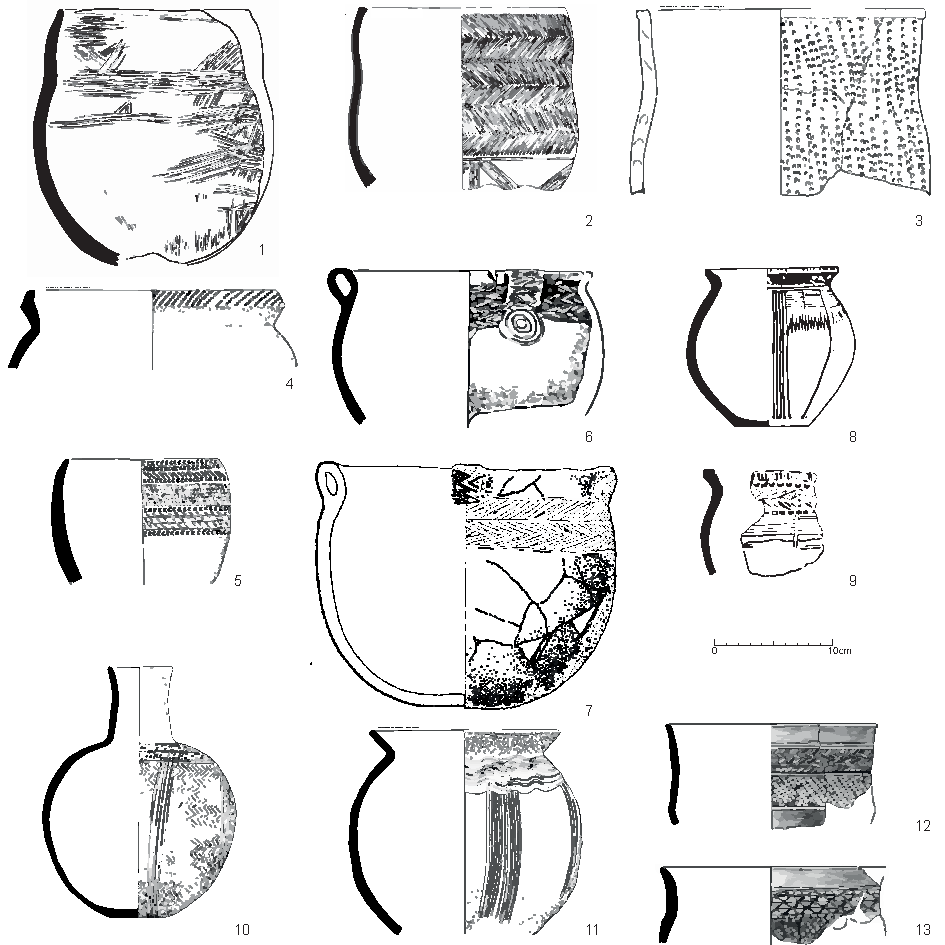
\includegraphics[width = \textwidth]{fig/Gabun_Typen.pdf}
	\caption{Gabun: Regionale Sequenz nach \textcite{Clist.20042005}.\\ 1--3: Okala-Gruppe \parencites[280 Abb.~6-71.2, 322 Abb.~6-105]{Clist.20042005}[187 Taf.~17.2]{Eggert.2016}; 4--5: Oveng-Gruppe \parencite[569 Abb.~7-25.1--2]{Clist.20042005}; 6--7: Okanda-Gruppe \parencites[355 Taf.~31.1]{AssokoNdong.20002001}[534 Abb.~6-230]{Clist.20042005}; 8--9: Otoumbi-Gruppe \parencite[626 Abb.~7-76.1, 7-76.3]{Clist.20042005}; 10--11: Nanda-Gruppe/\textit{Groupe II} \parencite[605 Abb.~7-49.2, 608 Abb.~7-52.2]{Clist.20042005}; 12--13: Angondje-Gruppe \parencite[224 Abb.~6-43]{SanchezElipe.2015}.}
	\label{fig:Gabon_Sequence}
\end{figure*}

Den Beginn der regionalen Sequenz bildet die in die letzte Hälfte des 1.~Jt. v.~Chr. datierte Okala-Gruppe \parencites{Clist.1988}{Clist.1997}[511]{Clist.20042005}. \textsc{Clist} (ebd. 489--511, 531--533) rechnet auch die Gruppen Epona \parencites{Oslisly.1992}{Oslisly.199495}{Oslisly.1998}{Oslisly.2001b}{Oslisly.1992b} und Yindo \parencites{AssokoNdong.20002001}{AssokoNdong.2002} des mittleren Ogooué-Tals der Okala-Gruppe zu. Die entsprechende Keramik zeichnet sich durch hohe, leicht geschweifte Grundformen mit flachen Böden und gerillten Ränder aus (Abb.~\ref{fig:Gabon_Sequence}.1--3). Eine Leitform der Okala-Gruppe bilden die sogenannten \textit{Bilobé}-Gefäße mit ihrem doppelt-halbkreisförmigem Profil \parencite[siehe][161 Abb.~3.3--4, 163 Anm.~3]{Seidensticker.2010c}. Die Verzierung besteht aus horizontalen Bändern aus feinem Kammstrich (Tab.~\ref{tab:Verzierungselemente}: 01.9--10) oder Fischgrätmustern (Tab.~\ref{tab:Verzierungselemente}: 01.7) sowie mit Kamm oder Klinge erzeugtem Wiegeband (Tab.~\ref{tab:Verzierungselemente}: 04.1--2). Grundsätzlich zählen zum Formenspektrum der Okala-Gruppe jene hohen Gefäße mit kurz ausbiegenden, gerillten Rändern und flächigem Kammwiegeband (Abb.~\ref{fig:Gabon_Sequence}.3), die für die in Südwestkamerun beschriebenen Stilgruppen Bissiang beziehungsweise Malongo charakteristisch sind (Kap.~\ref{sec:Kamerun}).\footnote{Das Inventar einer in Campo am Ntem im äußersten Südwesten Kameruns ausgegrabenen Grube (CAM~07/11) zeichnet sich durch \textit{Bilobé}-Gefäße, die die Leitform der Okala-Gruppe bilden (\textsc{Clist} 2004/2005: 489--500), sowie jene hohen, mit Kammwiegeband verzierten Gefäße aus, die in Südwestkamerun der Bissiang- beziehungsweise Malongo-Gruppe zugerechnet werden \parencites[330--341]{GouemGouem.20102011}[233--249]{NlendNlend.20132014}. Die beobachtete enge Vergesellschaftung dieser Merkmale unterstreicht die durch \textcites[632 Abb.~43.3]{deMaret.2013}[249 Abb.~113]{NlendNlend.20132014} vorgeschlagene Zusammenlegung der entsprechenden frühen Keramik in Kamerun und Gabun.} Die in den Inventaren des mittleren Ogooué-Tals ebenfalls enthalten Gefäße mit geschlossenem beziehungsweise schräg einbiegendem Rand \parencite[siehe][99 Abb.~5.B]{Oslisly.1998} spiegeln eine regionale Fazies der Okala-Gruppe wider. Die von \textcites{AssokoNdong.20002001}[142 Abb.~4]{AssokoNdong.2002} beschriebene und von \textcite[531--533]{Clist.20042005} der Okala-Gruppe zugeschlagene Yindo-Keramik aus der Lopé-Reservation umfasst tendenziell kleinere Gefäße mit umgelegten Rändern und einer Verzierung mit Appliquén. Die selben Inventare enthalten aber auch die bereits genannten, charakteristischen hohen Gefäße mit kurz umgelegten, gerillten Rändern und Kammwiegeband \parencite[186 Taf.~11,R.6]{AssokoNdong.20002001}.\footnote{Ebenfalls mit Kammwiegeband verzierte Scherben fanden sich auch an der Fundstelle Rivière Denis, deren vorliegende Datierungen leider stark streuen \parencite[438, 441 Abb.~6-187, 447 Abb.~6-194]{Clist.20042005}.} Die ältesten Zeugnisse für Eisenmetallurgie werden durch \textcite[202]{Oslisly.1992} von den Fundstellen Otoumbi 2 sowie Lopé 10 beschrieben und in das 8.--4. Jh. v.~Chr. datiert.

Auf die Okala-Keramik folgend lässt sich eine Regionalisierung der keramischen Entwicklung beobachten. Die ins 1--8.~Jh. n.~Chr. datierende und größtenteils auf das Umland von Libreville \parencite[615--618]{Clist.20042005} sowie die Äquatorialguinea vorgelagerte Insel Corisco \parencites{GonzalezRuibal.2011}{GonzalesRuibal.2012}{SanchezElipe.2015}{SanchezElipe.2016} beschränkte Oveng-Gruppe zeichnet sich durch Gefäße mit geschweifter Wandung und einfach ausbiegenden oder zylindrischen sowie kurzen, konvex ausbiegenden Rändern aus, die in einem zylindrischen oder einbiegenden Mündungsabschluss enden \parencites[Abb.~\ref{fig:Gabon_Sequence}.4--5;][559 Abb.~7-18]{Clist.20042005}[134 Abb.~15]{GonzalesRuibal.2012}. Das Spektrum an Verzierungen ist weiterhin von Rillen und Riefen sowie Kammeindrücken und Kammwiegeband bestimmt, während die Gefäßunterteile regelhaft frei von Verzierungen sind.\footnote{Die Oveng-Keramik aus dem nordwestlichen Gabun weist einige Parallelen zur Keramik der am unteren \mbox{Sangha} sowie dem 1987 befahrenen Abschnitt des Kongo verbreiteten Bokonongo-Gruppe auf (siehe Kap.~\ref{sec:BOG-Gr}).} Die Funde aus Corisco ließen eine Differenzierung der Oveng-Gruppe in drei Phasen zu: die Ältere vom 1.--5.~Jh. n.~Chr. ist ausschließlich in Gräbern belegt, während die mittlere Phase ausschließlich in Siedlungskontexten angetroffen wurde und in das 4.--6./7.~Jh.~n.~Chr datiert \parencites{SanchezElipe.2015}[354]{SanchezElipe.2016}. Die jüngere Phase umfasst eine Keramik, die formale Ähnlichkeiten zur mittleren Oveng-Keramik aufweist, aber frei von Verzierungen ist. Bislang wurde sie ausschließlich durch \textcites{SanchezElipe.2016} beschrieben und in das 7.--8.~Jh. n.~Chr. datiert. \textsc{Sánchez-Elipe} u.~a. (ebd. 355) bringen die späte Phase der Oveng-Gruppe mit einem potenziellen Bevölkerungsrückgang und damit verbundenem sozialen Verfall in Zusammenhang.

Die Okanda-Gruppe des mittleren Ogooué-Tals datiert ebenfalls in einen Zeitabschnitt zwischen der Mitte des 1. Jh. v.~Chr. und dem Ende des 5. Jh. n.~Chr. \parencite[619--622]{Clist.20042005}. Die bestimmende Gefäßform der Okanda-Gruppe sind hohe, beutelartige Gefäße mit nur leicht ausbiegenden Rändern (Abb.~\ref{fig:Gabon_Sequence}.6--7). Das Spektrum an Verzierungselementen umfasst neben Riefen und Rillen auch in Appliqué ausgeführte Muster. Vor allem unter dem Randabschluss ansetzende Henkel sind ein Charakteristikum der Okanda-Keramik \parencite[100 Abb.~6]{Oslisly.1998}. Ebenfalls in die Mitte des 1.--5. Jh. n.~Chr. datiert die lediglich in einem engen Gebiet um die eponyme Fundstelle im mittleren Ogooué-Tal verbreitete Keramik der Otoumbi-Gruppe \parencite[623--625]{Clist.20042005}. Sie zeichnet sich durch flachbodige Gefäße mit geschweifter Wandung und kurzen, ausbiegenden Rändern mit flach abgestrichener Randlippe aus (Abb.~\ref{fig:Gabon_Sequence}.8--9; ebd. 626 Abb.~7-67). Die Verzierung besteht vornehmlich aus Wiegeband im Halsbereich sowie Eindrücken auf der Randlippe und vertikalen sowie horizontalen Rillen auf der Wandung.

Auf die drei Gruppen Oveng, Okanda und Otoumbi folgt die Nandá-Gruppe \parencite[300 Anm.~4, 338--340]{SanchezElipe.2015}, die von \textcite[628--631, 628 Abb.~7-68]{Clist.20042005} noch als \textit{Groupe~II} bezeichnet wurde und in das 10.--12. Jh. n.~Chr. datiert \parencite[357]{SanchezElipe.2016}.\footnote{\textsc{Sánchez-Elipe} u.~a. (2016: 355\,f.) postulieren für die Äquatorialguinea vorgelagerte Insel Corisco einen Abbruch der Besiedlungssequenz im 8.--10.~Jh. n.~Chr. In dieser Phase sind weder Gräber noch Siedlungsbefunde bekannt.} \textcite{Clist.20042005} gibt für den Beginn der Nandá-Gruppe noch das 7.~Jh. n.~Chr. an, stützt sich dabei aber auf eine Datierung mit einem Standardfehler von $\pm$140 Jahren (Beta-20784), die von \textcites[357]{SanchezElipe.2016} als nicht repräsentativ angesehen wird. Neben wenigen Fundstellen in der Region um Libreville \parencite[629 Abb.~7-69]{Clist.20042005} fand sich Keramik der Nandá-Gruppe auch auf der im Grenzgebiet zu Äquatorialguinea gelegenen Insel Corisco. Sie zeichnet sich durch Flaschen mit stark geschweifter Wandung und langen, zylindrischen Hälsen sowie einfach ausbiegenden Rändern aus \parencites[Abb.~\ref{fig:Gabon_Sequence}.10--11; ebd. 603--611 Abb.~7-47--7-55;][222 Abb.~6.41, 303--315 Abb.~7.46--7.58]{SanchezElipe.2015}[137 Abb.~18]{GonzalesRuibal.2012}. Die Wandungen der Nandá-Keramik sind häufig mit vertikalen Bändern aus parallelem Kammstrich oder Fischgrät-Muster verziert, während Ränder und Unterteile teilweise unverziert sind. Ein großer Teil der von Clist noch als \textit{Groupe~II} bezeichneten Nandá-Keramik stammt von der Fundstelle Sablière bei Libreville \parencite[600--614]{Clist.20042005} und der Insel Corisco \parencites{GonzalezRuibal.2011}{GonzalesRuibal.2012}.

Im Umland von Libreville folgt auf die Nandá-Keramik die Angondjé-Gruppe, die mit den ersten europäischen Kontaktfunden, unter anderem Tabakpfeifen, zusammenfällt. Die Assoziation mit diesen Importen liefert auch einen \textit{terminus ante quem} für die von \textcite[691]{Clist.20042005} in das 10.--16. Jh. n.~Chr. datierte Angondjé-Keramik \parencites[siehe][224]{SanchezElipe.2015}[357\,f.]{SanchezElipe.2016}. Funde der Angondjé-Gruppe fanden sich vornehmlich im Umland von Libreville, im Nordwesten Gabuns \parencite[692 Abb.~7-122]{Clist.20042005}. Die Angondjé-Keramik zeichnet sich durch rundbodige Schalen mit scharfem Bauchknick aus \parencite[Abb.~\ref{fig:Gabon_Sequence}.12--13; ebd. 645--649 Abb.~7.81--7.85; ][187 Abb.~6.20, 223--224 Abb.~6.42--6.43]{SanchezElipe.2015}, die grundsätzliche Ähnlichkeiten zu den entsprechenden Schalen des Typs F3 der Stilgruppen Pikunda-Munda (Kap.~\ref{sec:PKM-Gr}) sowie Mobaka (Kap.~\ref{sec:MKA-Gr}) aus dem Arbeitsgebiet zeigen. Die Schalen der Angondjé-Gruppe weisen oberhalb des Bauchknicks häufig eine Ritzverzierung aus diagonalen bis schachbrettartigen Mustern und Eindrücke auf. 